\section[Intro classif.]{Introduction}
\begin{frame}
\frametitle{Differentiate between groups of patients}
Classification (or prediction if a continuous variable)

\vspace*{30pt}

A classical problem in statistics and machine learning.  

\vspace*{30pt}

What do we want? A good classifier. Something that, given a new sample,
will assign it to its appropriate group.

\end{frame}
 

\begin{frame}
\frametitle{}
\TPMargin{3pt}
\textblockcolour{red}
%%\textblockrulecolour{red}
\begin{textblock*}{103mm}(23mm,25mm)
  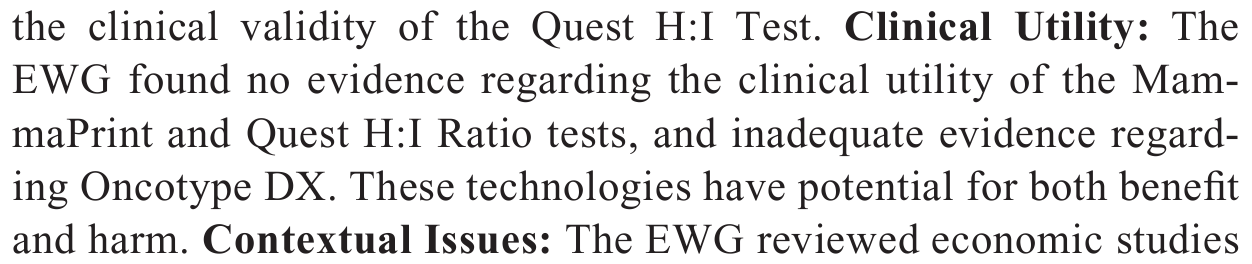
\includegraphics[%
  width=10.1cm,
  keepaspectratio]{detail-egapp.png}
\end{textblock*}
\textblockcolour{white}
\TPMargin{3pt}
\textblockcolour{black}
%%\textblockrulecolour{red}
\begin{textblock*}{102mm}(20mm,3.7mm)
  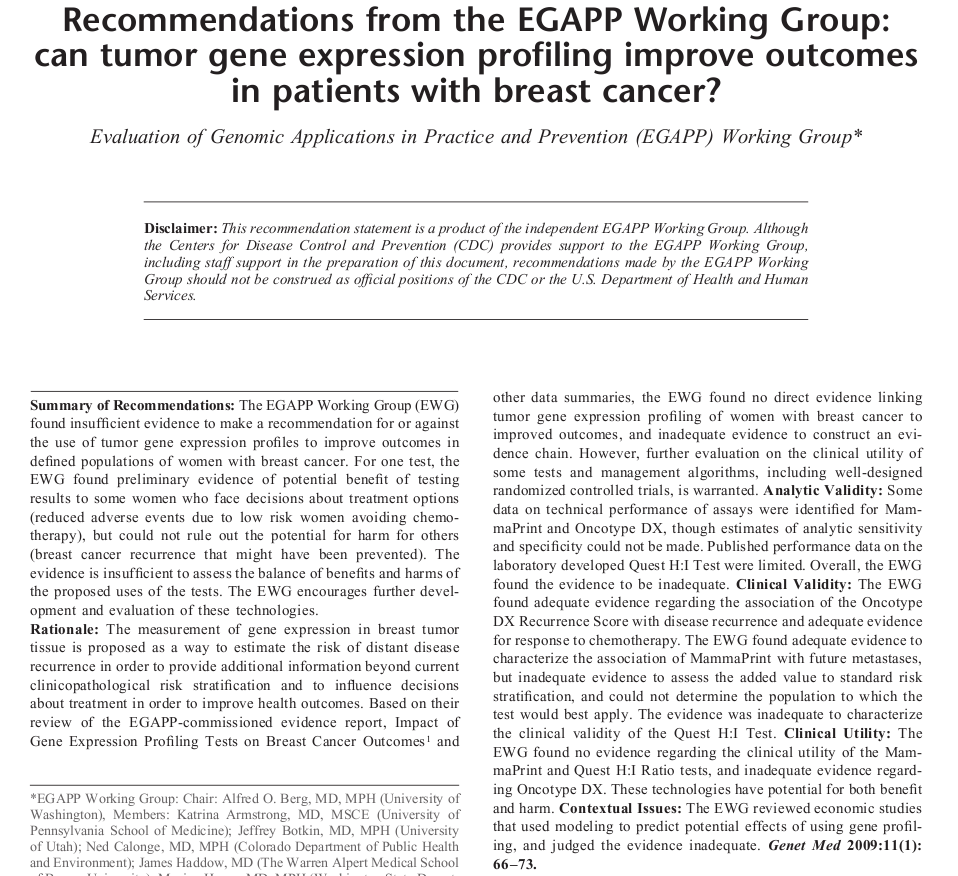
\includegraphics[%
  width=10.0cm,
  keepaspectratio]{egapp.png}
\end{textblock*}
\textblockcolour{white}
\textblockcolour{red}
%%\textblockrulecolour{red}
\begin{textblock*}{103mm}(23mm,25mm)
  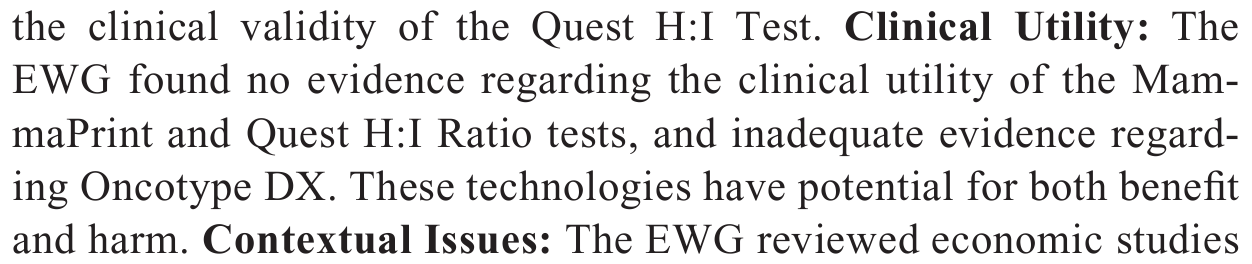
\includegraphics[%
  width=10.1cm,
  keepaspectratio]{detail-egapp.png}
\end{textblock*}
\textblockcolour{white}
\textblockcolour{white}
\note[item]{Decepcionante, dado el dinero y número de estudios.}
\note[item]{La promesa de las ``ómicas'': medicina individualizada}
\end{frame}


\begin{frame}
\frametitle{\ldots clinical utility}
{\footnotesize
  \begin{description}
  \item[Clinical validity] predict risk of recurrence
  \item[Clinical utility] predict benefit of a treatment over another: added
    value when making decissions.
  \end{description}
}

\vspace*{20pt}

\begin{itemize}
  
\item \ldots when we already have conventional classifiers/predictors
  
  \vspace*{20pt}
  
\item \textbf{Does the new method/algorithm, based on genomic data,
    improve our ability to predict a result, compared to what we could
    predict without those genomic data?}
  
\end{itemize}
\end{frame}

\begin{frame}
\frametitle{The dangers of ``capitalizing on chance}

Statistical context: many genes, few subjects. $p \gg n$.


\note[item]{La estadística es, en gran parte, la ciencia que nos alerta contra
  esas capitalizaciones. La que nos explica que las coincidencias son,
  eso, coincidencias y no evidencias de nada.}

\begin{description}
\item[Differentially expressed genes] Risk of too many false positives
  $\Rightarrow$ adjustments in the screening of p-values.
  
  
  \vspace*{20pt}
\item[Classification/prediction] Very easy to obtain algorithms that
  classify, perfectly, our data, but not new data
  $\Rightarrow$ validate algorithms and classifiers
  
  
  \vspace*{20pt}
\item[Hypotheses/questions] Tempting to make them vague, or ask none and
  wait until ``the data say something'' $\Rightarrow$ define objectives
  and how we will measure what we are interested in.
  
  \note[item]{por esto último NO hablaremos de clustering}
  \note[item]{Los datos siempre confiesan si los torturamos lo suficiente}
  \note[item]{Con muchos datos, no hace falta mucha tortura}
  % \begin{itemize}
  % \item p-valores no interpretables
  % \item calidad predictiva modelo no suele mejorar
  % \end{itemize}
  
\end{description}
\end{frame}



\subsection{References}

\begin{frame}
\frametitle{Review of methods and good practices.}

(***): highly recommended
\begin{itemize}
  
\item Tarca et al., 2013.   Strengths and limitations of microarray-based
  phenotype prediction: lessons learned from the IMPROVER Diagnostic
  Signature Challenge. \textit{Bioinformatics}, 29: 2892--2899. (***)
\item Shi et al. 2010. The MicroArray Quality Control (MAQC)-II study of
  common practices for the development and validation of microarray-based
  predictive models. \textit{Nature Biotechnology}, 28: 827--838. (***)

  
\item   Dupuy A, Simon R. 2007. Critical Review of Published Microarray Studies
  for Cancer Outcome and Guidelines on Statistical Analysis and
  Reporting. \textit{J Natl Cancer Inst.}, 99: 147--157.  (***)
\end{itemize}
\end{frame}


\begin{frame}
\frametitle{Books}
\begin{itemize}
  \item Kuhn, and Johnson. 2013. Applied Predictive
    Modeling. \textit{Springer}. (***)
  \item James et al. 2013. An introduction to statistical
    learning. \textit{Springer}. (***) (A PDF can be downloaded freely and
    legally from their web page)
\end{itemize}
\end{frame}



\begin{frame}
\frametitle{}
\begin{itemize}
  \item Lee et al., 2005. \textit{Computational Statistics and Data
    Analysis}, 48: 869--885.
  
\item Zucknick et al. 2008. \textit{Stat Appl Genet Mol Biol.} 7 (se
  encuentra en la web, en PubMed central). 

\item Many other (see outdated list in Diaz-Uriarte, 2005.
  \Burl{http://ligarto.org/rdiaz/Papers/chapter-azuaje-dopazo.pdf}).
\item Slawski et al., \textit{BMC Bioinformatics}, 2008, 9:
  439. Description of many methods in a single paper. But it is not a comparison.

\item Dudoit, S., J. Fridlyand, and T. P. Speed. 2002.
    Comparison of discrimination methods for the classification of tumors suing gene expression data.
    \textit{J Am Stat Assoc} 97(457), 77-87. (You can find the reprint on
    the web.).

\end{itemize}
\end{frame}





\subsection{Key ideas}
\begin{frame}
\frametitle{Classification/prediction: key ideas}
\begin{itemize}
\item All we care about is a good classifier.
\item We do not care about p-values.
\item We will have to choose some genes.
\item We will have to, ESPECIALLY, estimate the error of the classifier.
\end{itemize}
\end{frame} 


\begin{frame}
\frametitle{Tell me how it works (dime c\'omo funciona) \ldots}
\begin{textblock*}{90mm}(25mm,16mm)
  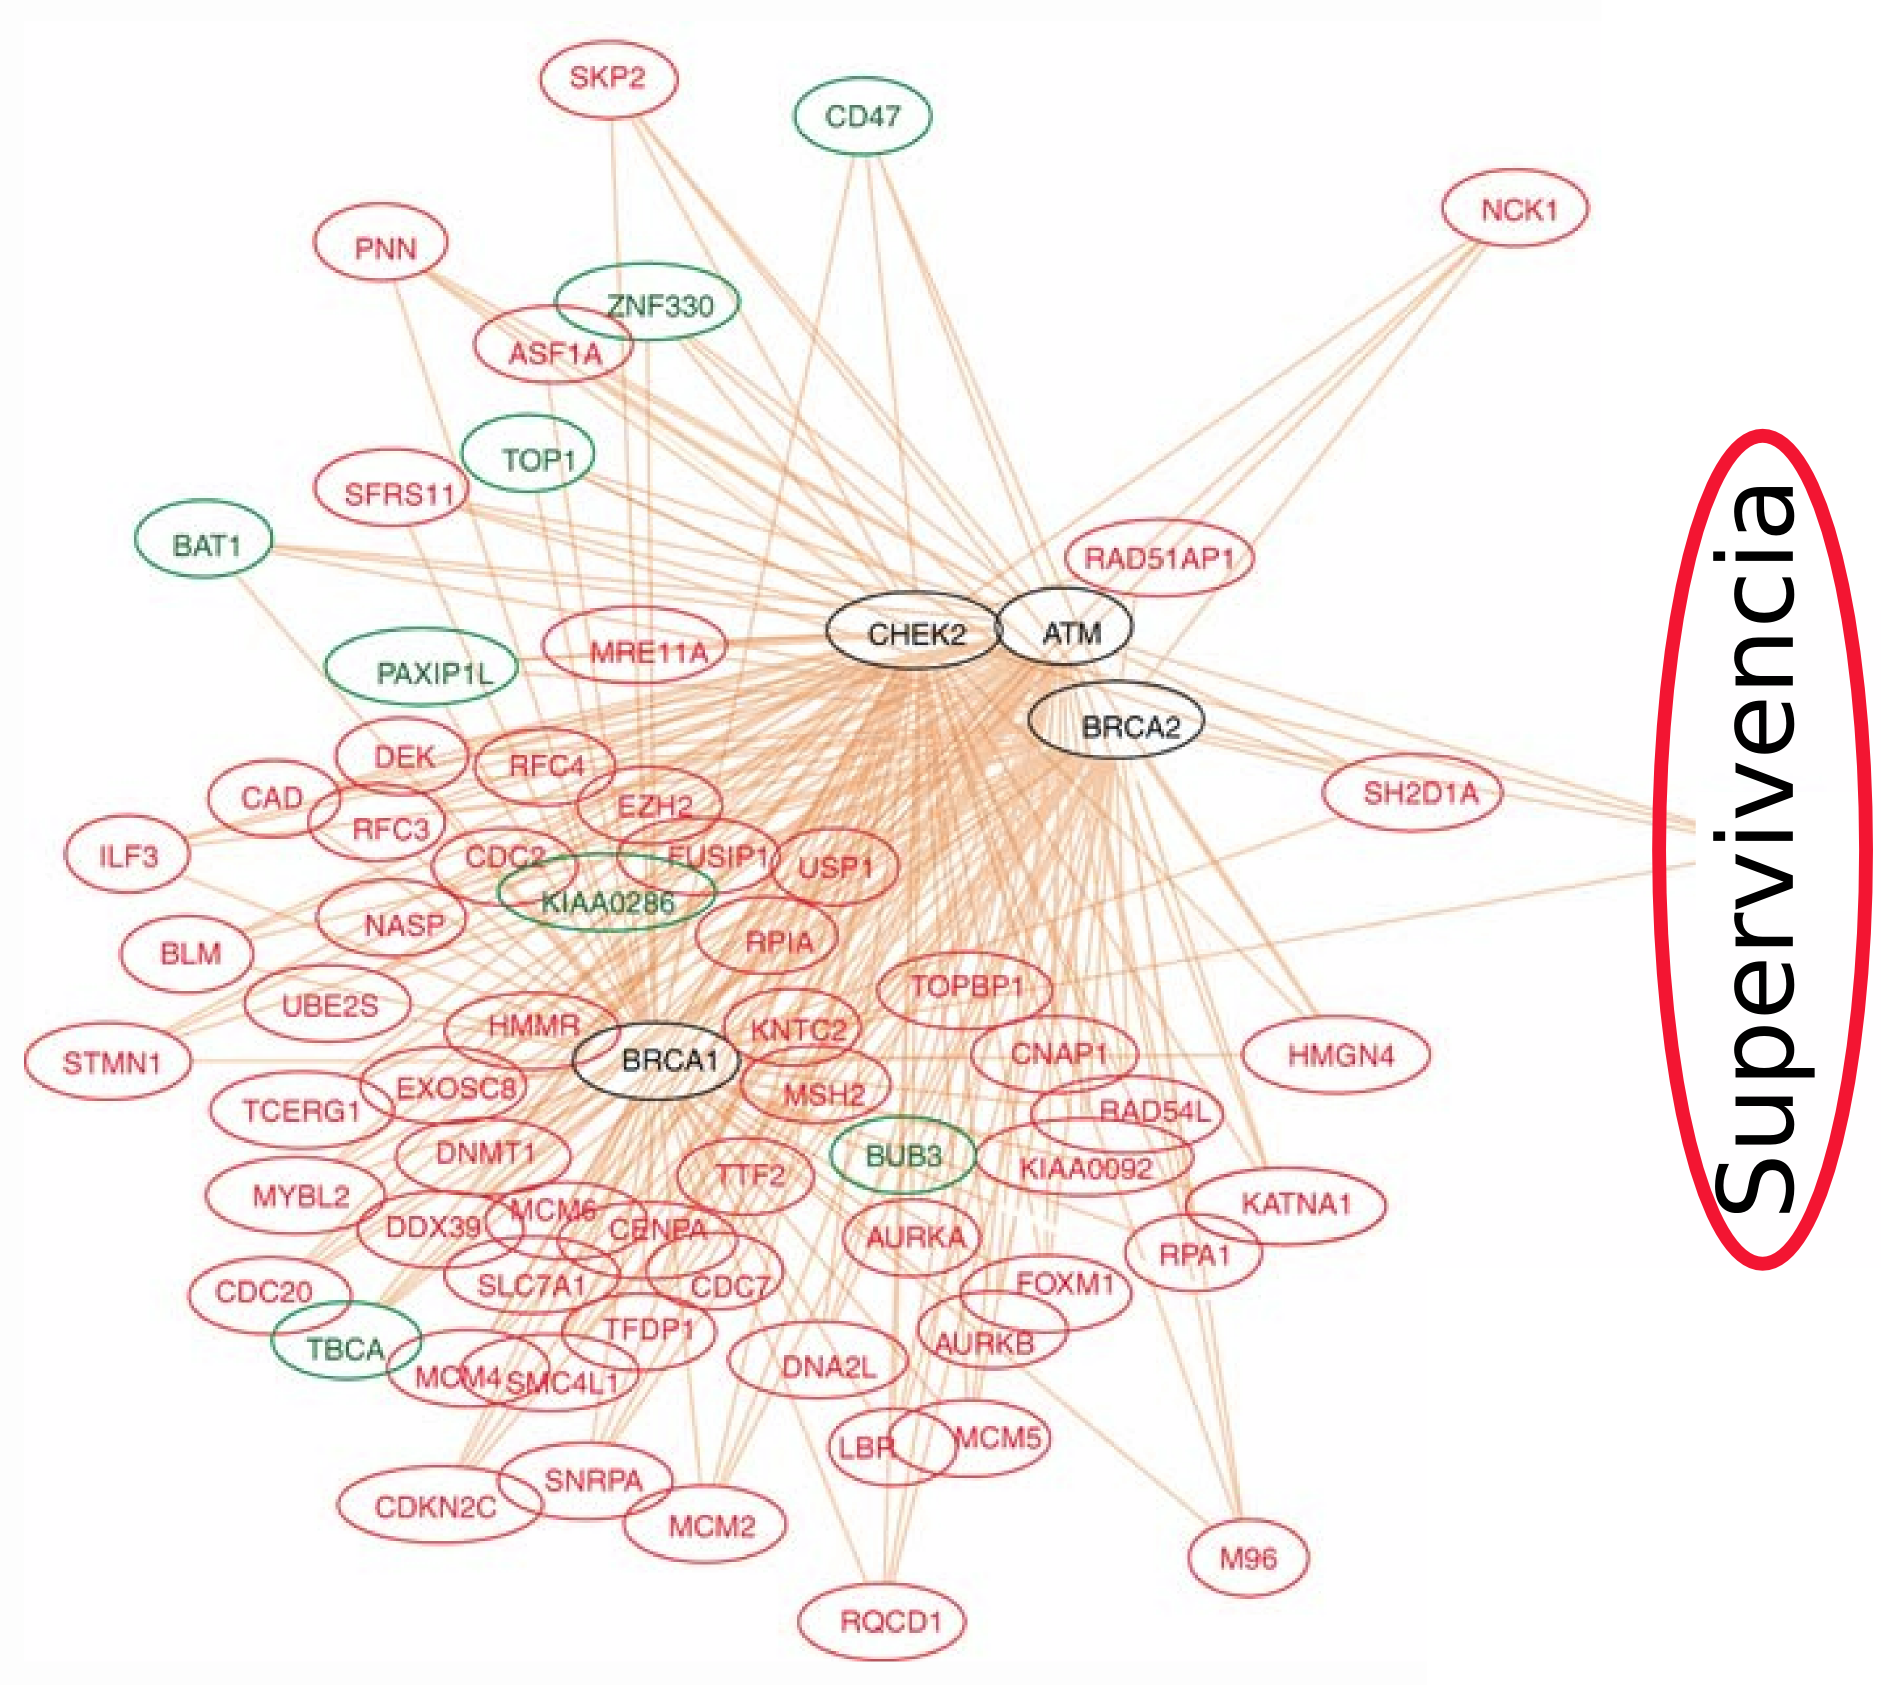
\includegraphics[%
  width=8.0cm,
  keepaspectratio]{white-box.png}
\end{textblock*}
\textblockcolour{white}
  \begin{textblock*}{53mm}(22mm,87mm)
    {\tiny(Modified from Pujana et al., 2007. Nat Genet. 39)}
  \end{textblock*}
\end{frame}



\begin{frame}
\frametitle{\ldots vs.\ the black box}
\begin{textblock*}{103mm}(13mm,20mm)
  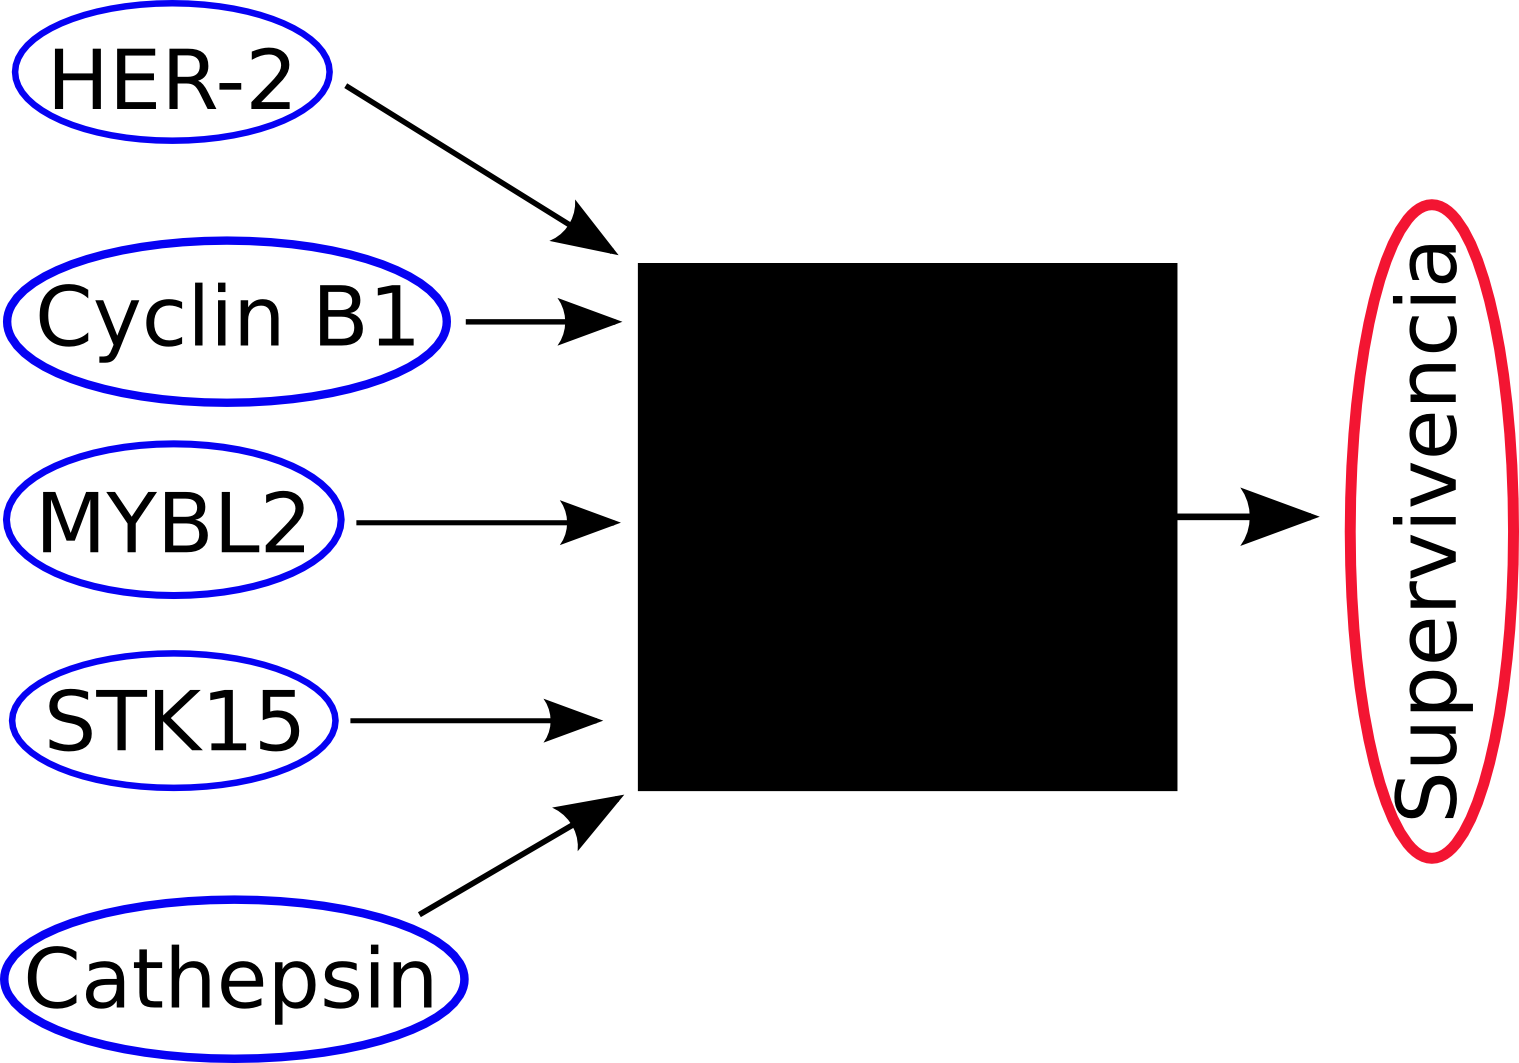
\includegraphics[%
  width=10.3cm,
  keepaspectratio]{black-box.png}
\end{textblock*}
\end{frame}




\begin{frame}
\frametitle{Prediction: black box}
\begin{itemize}
\item Rules of the game: that it predicts (classifies) well.
\vspace*{20pt}
\item We are not assessing the ``truth'' of the model. Only its predictive
  success.


\vspace*{20pt}
\item Almost all methods eliminate genes with redundant info for
  classification: this limits interpretability anyway.

\note{Input y Output: que prediga bien.}


\end{itemize}
\end{frame}





\begin{frame}
\frametitle{Prediction vs.\ interpretability}
\begin{itemize}
\item Good classifiers need not be intuitively easy to understand.
\item $p \gg n$: many classifiers with similar predictive capacity but
  different genes.
  
\item Black boxes ameliorate these problems (you do not worry too much
  about them).
\begin{itemize}
\item Inversions in the signs of coefficients
\item Genes shared between models
\end{itemize}
\vspace*{20pt}
\item Do not jump between objectives: classify vs.\ interpret.
\end{itemize}

\end{frame}









%%\subsection{Etapas}

\begin{frame}
\frametitle{Steps in the construction of a classifier with genomic data}
\begin{itemize}
\item Selection of a classification algorithm.
\item Gene selection.
\item Classifier construction/training.
\item Estimate the error of the classifier.
\end{itemize}
\end{frame}




\section[Algorithms]{Methods/Models/Algorithms for classification}
\subsection{Algorithms}
\begin{frame}
\frametitle{Some algorithms/models}
\begin{itemize}
\item Just to say some specific.
\item We will mention a few that work well.
\item There are lots we say nothing about.
\item ``Follow the pros'': read reviews, follow recommendations, and
  understand the methods you use.
\end{itemize}
\end{frame}


\begin{frame}
\frametitle{Reviews of methods.}
\begin{itemize}
  
  \item Malley et al., 2011. Statistical learning for biomedical
    data. \textit{Cambridge University Press}.
    
\item Shi et al. 2010. The MicroArray Quality Control (MAQC)-II study of
  common practices for the development and validation of microarray-based
  predictive models. \textit{Nature Biotechnology}, 28: 827--838.

  
% \item Dudoit, S., J. Fridlyand, and T. P. Speed. 2002.
%     Comparison of discrimination methods for the classification of tumors suing gene expression data.
%     \textit{J Am Stat Assoc} 97(457), 77-87. (You can find the reprint on
%     the web.).

%   \item Lee et al., 2005. \textit{Computational Statistics and Data
%     Analysis}, 48: 869--885.
  
  
% \item Statnikov et al. 2005. \textit{Bioinformatics}, 21 (5):
%   631--643. Where is DLDA???
% \item Zucknick et al. 2008. \textit{Stat Appl Genet Mol Biol.} 7 (se
%   encuentra en la web, en PubMed central). 
  
\end{itemize}
\end{frame}

% \begin{frame}
% \frametitle{}
% \begin{itemize}
% \item Many other (see outdate list in Diaz-Uriarte, 2005.
%   \Burl{http://ligarto.org/rdiaz/Papers/chapter-azuaje-dopazo.pdf}).
% \item Slawski et al., \textit{BMC Bioinformatics}, 2008, 9:
%   439. Description of many methods in a single paper. But it is not a comparison.
% \end{itemize}
% \end{frame}



\begin{frame}
\frametitle{A great presentation}

\Burl{http://www-onderzoek.lumc.nl/HumaneGenetica/mgc/2005/presentations/Classification_Wessels.pdf}
\end{frame}







\begin{frame}
\frametitle{Nearest mean}
\begin{itemize}
\item As it says: the closest mean
\item (Next two slides from {\tiny\Burl{http://www-onderzoek.lumc.nl/HumaneGenetica/mgc/2005/presentations/Classification_Wessels.pdf}})
\end{itemize}
\end{frame}


\begin{frame}
\frametitle{}
\begin{center}
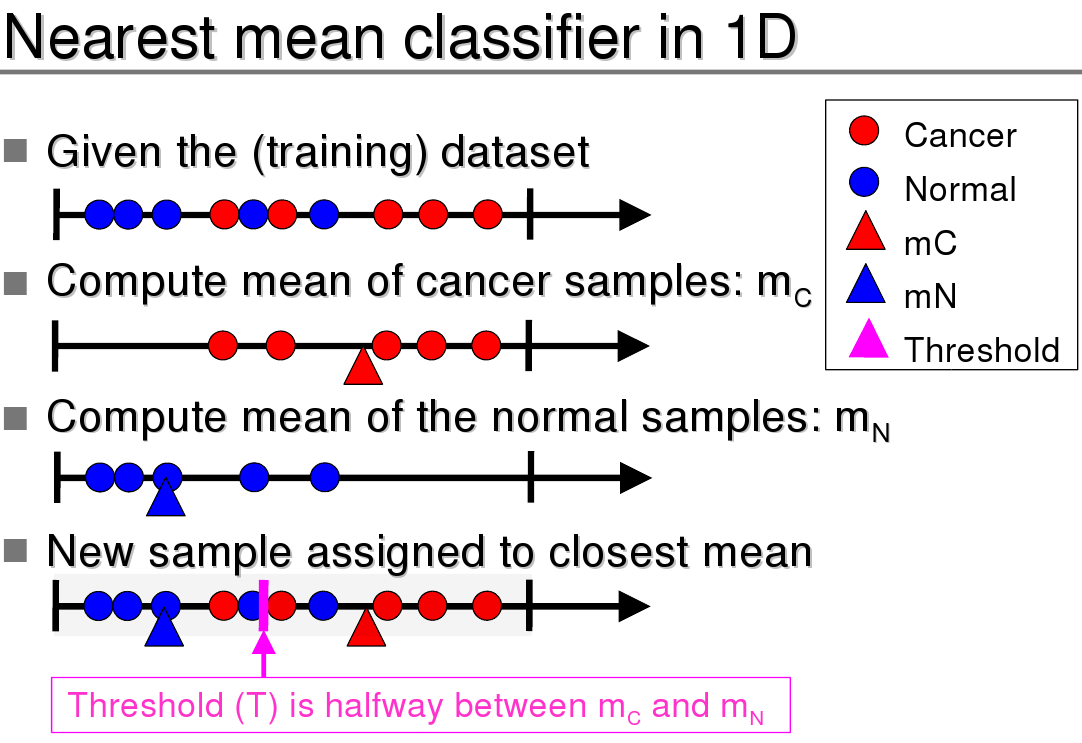
\includegraphics[%
    width=10.0cm,
    keepaspectratio]{wess1.png}
\end{center}
(Taken from Lodewyk Wessels, Classification\_Wessels.pdf)
\end{frame}

\begin{frame}
\frametitle{}
\begin{center}
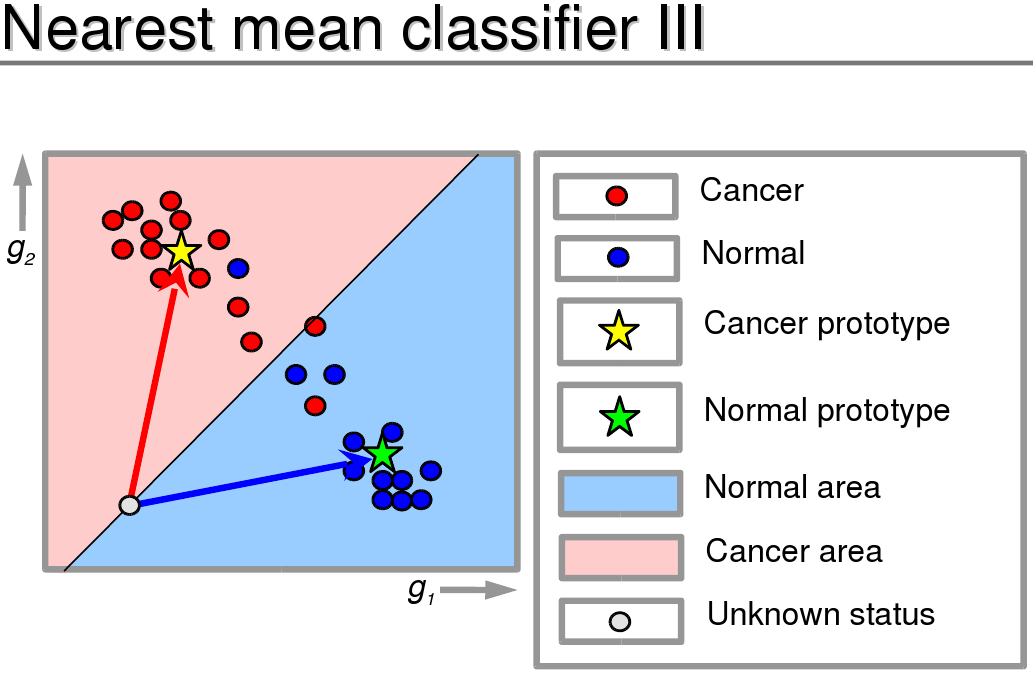
\includegraphics[%
    width=10.0cm,
    keepaspectratio]{wess2.png}
\end{center}
(Taken from Lodewyk Wessels, Classification\_Wessels.pdf)
\end{frame}



\begin{frame}
\frametitle{KNN}
\begin{itemize}

\item K-nearest neighbor.

\item Simple non-parametric rule:

\item Predicts the sample of a test case as the majority vote
among the k nearest neighbors of the test case.

\item To decide on ``nearest'' we often use
the Euclidean distance, but other measures of proximity are possible. 

\item The number of neighbors used (k) is either fixed or chosen
by cross-validation.
\end{itemize}

\end{frame}


\begin{frame}
\frametitle{}
\begin{center}
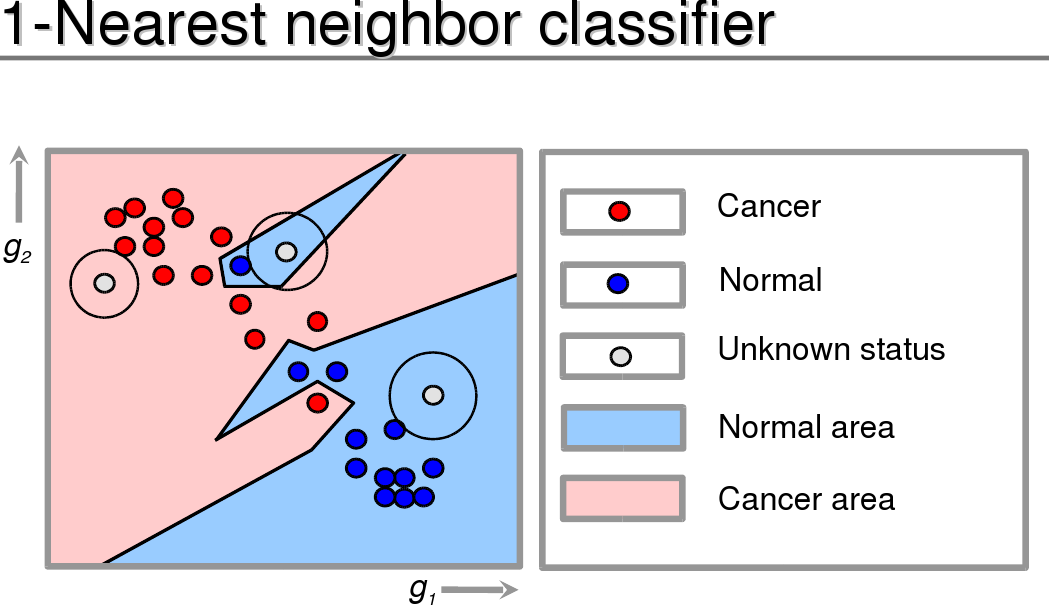
\includegraphics[%
    width=10.0cm,
    keepaspectratio]{wess3.png}
\end{center}
(Taken from Lodewyk Wessels, Classification\_Wessels.pdf)
\end{frame}



\begin{frame}
\frametitle{DLDA}
\begin{itemize}
\item Diagonal Linear Discriminant Analysis.

\item A form of discriminant analysis (optimal when class densities have the same diagonal 
variance-covariance matrix).

\item Simple linear rule:  a sample is
assigned to the class $k$ which minimizes 
$\Sigma_{j = 1}^p (x_j - \bar{x}_{kj})^2/\hat{\sigma}^2_j$,
where $p$ is the number of variables, $x_j$ is the value on variable (gene) $j$ of the test
sample, $\bar{x}_{kj}$ is the sample mean of class $k$
and variable (gene) $j$, and $\hat{\sigma}^2_j$ is
the (pooled) estimate of the variance of gene $j$.
\item Unrealistic assumption, but works very well (and often better than other
  forms of discriminant analysis that require estimation of many more
  parameters).

\item Also called ``Naïve Bayes.''

\end{itemize}



\end{frame}

\begin{frame}
\frametitle{Random Forest}
\begin{itemize}
\item An ensemble of classification trees.

\item Each tree is grown using a
bootstrap sample of the data set, and at each node only a random
subset of the original variables is examined.

\item Interactions are implicitly considered.

\item Provides ranking of variable importance.
\end{itemize}
\end{frame}



\begin{frame}
\frametitle{Logistic regression}
\begin{itemize}
\item We model the (logit of the) probability of belonging to a class as a linear
combination of features. Extension of linear models to binary data.

\item As well as DLDA, this is a ``classic'' of statistics.

\end{itemize}

\end{frame}


\begin{frame}
\frametitle{SVM}
\begin{itemize}
\item Support vector machines.

\item Obtain the best separating hyperplane between classes; hyperplane is located
so that it has maximal margin (i.e., so that there is maximal distance between the
hyperplane and the nearest point of any of the classes). 

\item When the data not separable,
there is no separating hyperplane; in this case, we still try to maximize the margin
but allow some classification errors subject to the constraint that
the total error (distance from the hyperplane in the ``wrong side'') is
less than a constant.
\end{itemize}
\end{frame}



\begin{frame}
\frametitle{}
SVM: separable case
\begin{center}
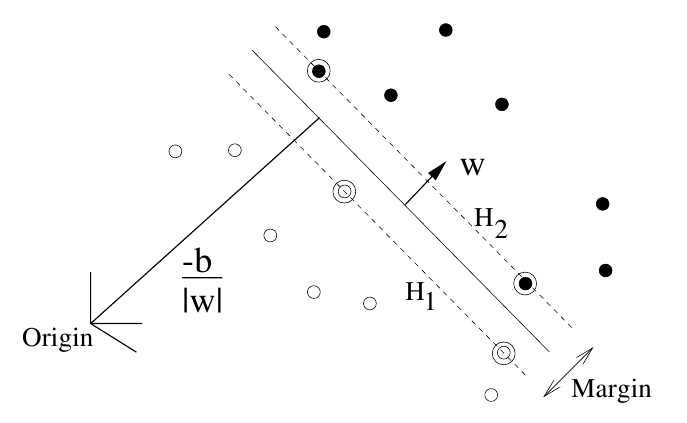
\includegraphics[%
    width=10.0cm,
    keepaspectratio]{svm1.png}
\end{center}
{\small (Taken from Burgues, 1998, \textit{Data Mining and Knowledge Discovery} 2, 121-167)}
\end{frame}


\begin{frame}
\frametitle{}
SVM: non-separable case
\begin{center}
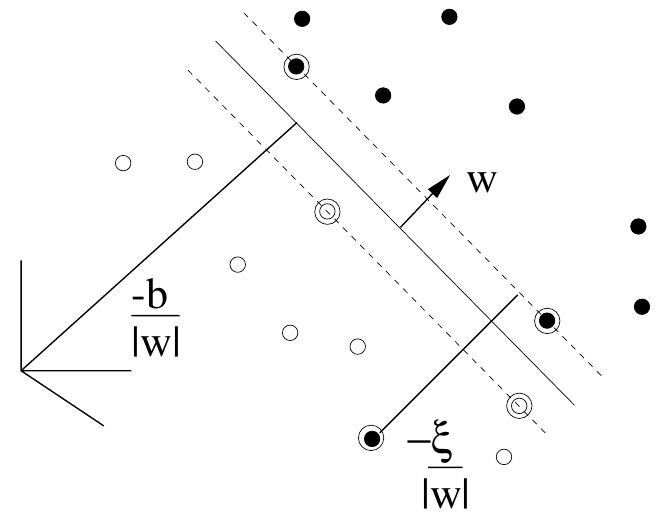
\includegraphics[%
    width=9.0cm,
    keepaspectratio]{svm2.png}
\end{center}
{\small (Taken from Burgues, 1998, \textit{Data Mining and Knowledge Discovery} 2, 121-167)}
\end{frame}



\subsection{Gene selection}
\begin{frame}
\frametitle{Gene selection}
\begin{itemize}
\item Filter approaches: select before training the classifier.
\begin{itemize}
\item Univariate
\item Multivariate
\end{itemize}
\item Wrapper approaches. Within the classifier. A few infamous examples:
   stepwise regression et al. (There are non-infamous examples too).
\end{itemize}
\end{frame}


\section[Error estimation]{Estimating the classifier's error}
\begin{frame}
\frametitle{Estimating the classifier's error (or ``validating the classifier'')} 

A sample with 50 healthy subjects and 50 diseased ones.

We build a classifier with those 100 samples, and on those 100 we make a
mistake of 10\%.
\pause
\vspace*{30pt}

Can we use that 10\% as a reasonable estimate of the error we would make
with new samples?
\end{frame}


% \begin{frame}
% \frametitle{}
% \begin{center}
% 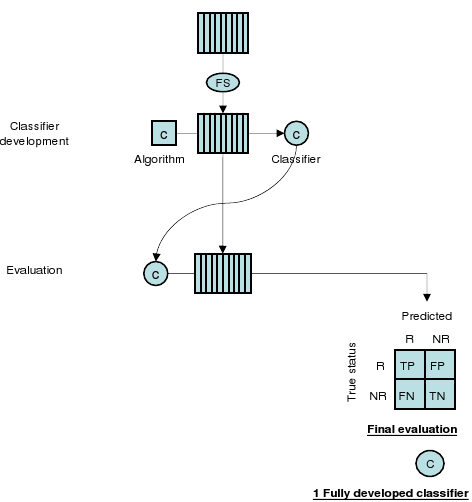
\includegraphics[%
%     width=7.0cm,
%     keepaspectratio]{dupuy1.png}
% \end{center}
% (From Dupuy and Simon, 2007)

% \end{frame}



\begin{frame}
  \frametitle{Resubstitution}
  \vspace*{-5cm}
%  \centerline{``Split-sample'', ``holdout validation'', ``data splitting''}
   \textblockcolour{}
  \TPMargin{0pt}
  \begin{textblock*}{75mm}(20mm,15mm)
    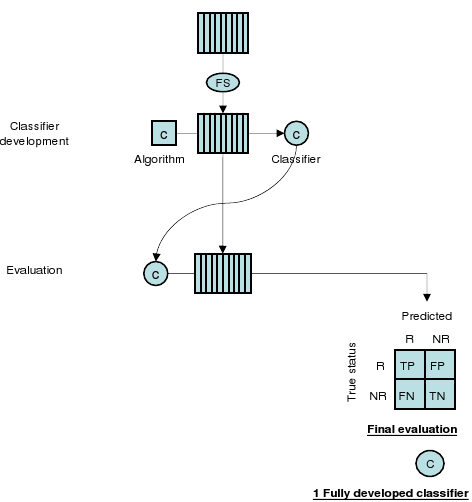
\includegraphics[%
    width=7.50cm,
    keepaspectratio]{dupuy1.png}
  \end{textblock*}
  \begin{textblock*}{43mm}(27mm,92mm)
    \textblockcolour{}
    {\tiny(Dupuy and Simon, 2007, JNCI, 99)}
  \end{textblock*}
   \textblockcolour{}
\end{frame}



\begin{frame}
  \frametitle{``Split-sample'', ``holdout validation'', ``data splitting''}
  \vspace*{-5cm}
%  \centerline{``Split-sample'', ``holdout validation'', ``data splitting''}
  
  \TPMargin{0pt}
  \textblockcolour{black}
  %% \textblockrulecolour{red}
  \begin{textblock*}{75mm}(20mm,15mm)
    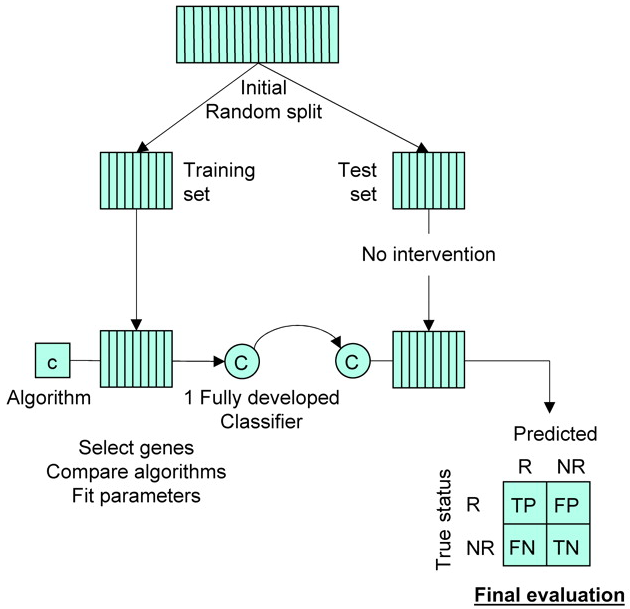
\includegraphics[%
    width=7.5cm,
    keepaspectratio]{ds1.png}
  \end{textblock*}
  \textblockcolour{white}
  \begin{textblock*}{43mm}(27mm,92mm)
    {\tiny(Dupuy and Simon, 2007, JNCI, 99)}
  \end{textblock*}
  
\note[item]{Random allocation}
\end{frame}



\begin{frame}
  \frametitle{``Cross-validation''}
  \vspace*{-5cm}
 % \centerline{``Cross-validation'' (bootstrap, etc)}
  
  \TPMargin{0pt}
  \textblockcolour{black}
  %% \textblockrulecolour{red}
  \begin{textblock*}{75mm}(20mm,15mm)
    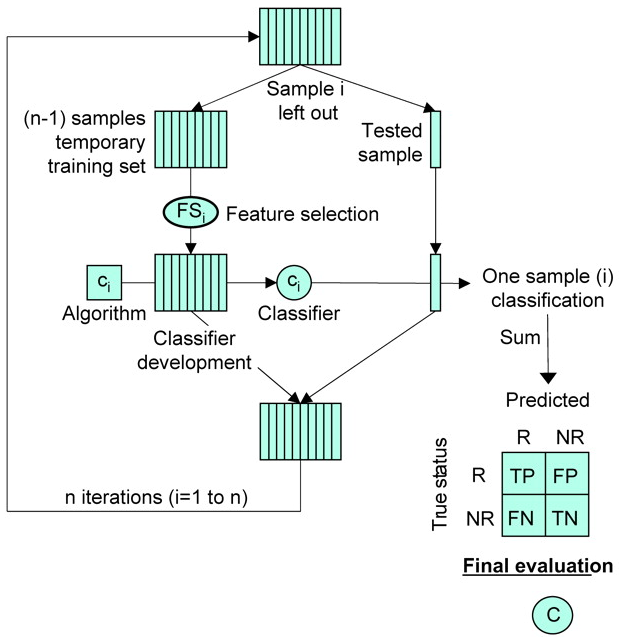
\includegraphics[%
    width=7.5cm,
    keepaspectratio]{ds2.png}
  \end{textblock*}
  \textblockcolour{white}
  \begin{textblock*}{43mm}(27mm,92mm)
    {\tiny(Dupuy and Simon, 2007, JNCI, 99)}
  \end{textblock*}

\note[item]{Ojo: tested NUNCA son vistos en training}
  
\end{frame}


\begin{frame}
\frametitle{}
\begin{itemize}
\item Suppose 100 subects, 50 healthy, 50 diseased.
\item Select at random 10 (``testing set'').
\item Usae the other 90 to build the classifier (``training set'').
\item Evaluate the classifier with the first 10.
\item Repeat the process another 9 times (until all subjects have been
  used exactly once in the ``testing set'').
\item We have 10 estimates of error, we compute the mean, and we now have
  an estimate of the error we would make with a new sample.
\end{itemize}
\end{frame}



\begin{frame}
  \frametitle{Cross-validation (3-fold, here)}
  \vspace*{-5cm}
  %% \textblockrulecolour{red}
  \begin{textblock*}{75mm}(10mm,25mm)
    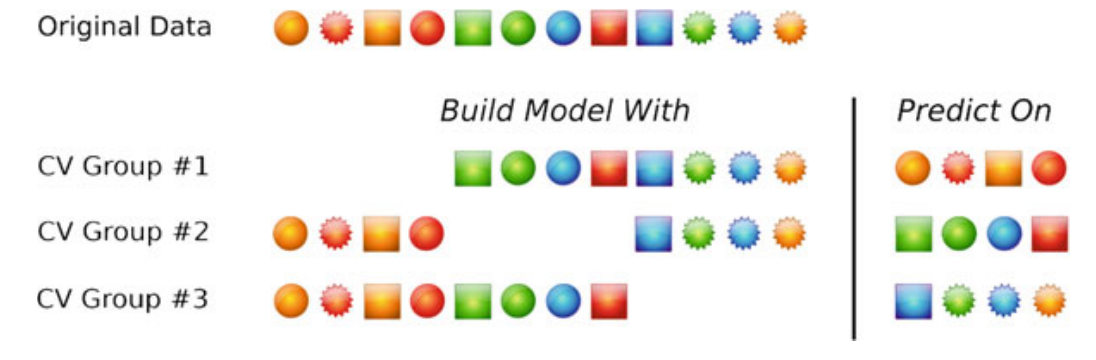
\includegraphics[%
    width=11.5cm,
    keepaspectratio]{cv-3-kuhn.png}
  \end{textblock*}
  \begin{textblock*}{83mm}(27mm,82mm)
  \textblockcolour{white}
    {\tiny(Kuhn and Johnson, 2013. \textit{Applied predictive modeling}, Springer}
  \end{textblock*}
 
\end{frame}


\begin{frame}
  \frametitle{Bootstrap}
  \vspace*{-5cm}
  \begin{textblock*}{75mm}(10mm,25mm)
    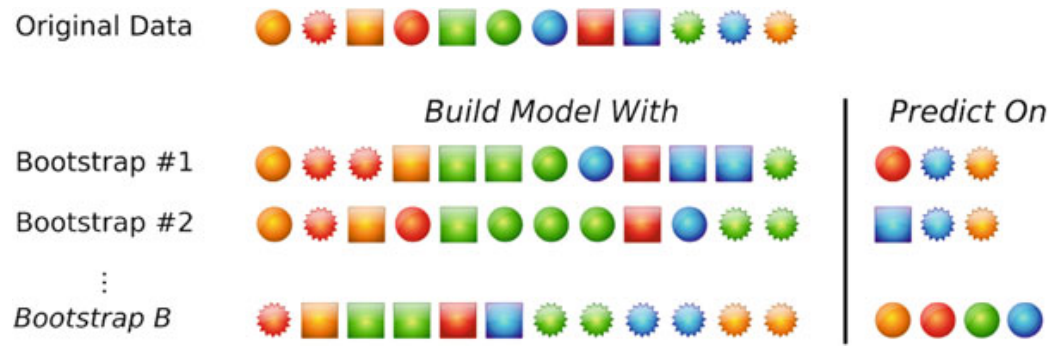
\includegraphics[%
    width=11.5cm,
    keepaspectratio]{boot-kuhn.png}
  \end{textblock*}
  \textblockcolour{white}
  \begin{textblock*}{83mm}(27mm,82mm)
    {\tiny(Kuhn and Johnson, 2013. \textit{Applied predictive modeling}, Springer}
  \end{textblock*}
\end{frame}




\begin{frame}
\frametitle{Independent validation}
Independent validation, with other samples, by other groups: necessary
\end{frame}




% \begin{frame}
% \frametitle{Validación cruzada}
% \begin{center}
% \includegraphics[%
%     width=6.5cm,
%     keepaspectratio]{dupuy2.png}
% \end{center}
% (From Dupuy and Simon, 2007)
% \end{frame}



\begin{frame}
\frametitle{Beware of ``selection bias''}
What if we have done gene selection?

\begin{itemize}
\item Select the 100 genes with smallest p-value.
\item Build the classifier.
\end{itemize}
\end{frame}


\begin{frame}
\frametitle{}
The validation process has to include the gene selection procedure.
We must do the gene selection in each training set.
\end{frame}




% \begin{center}
% 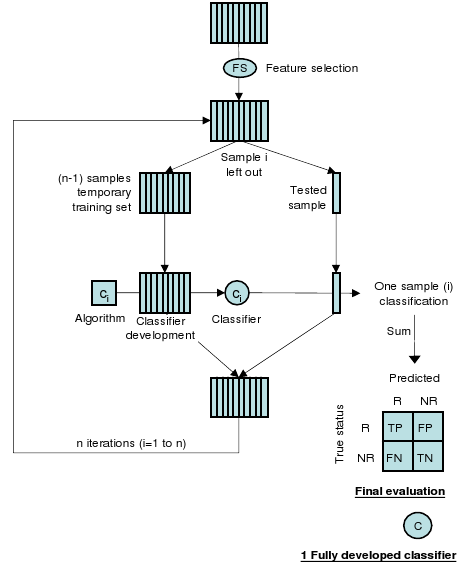
\includegraphics[%
%     width=5.5cm,
%     keepaspectratio]{dupuy3.png}
% \end{center}
% (From Dupuy and Simon, 2007)
% \end{frame}


\begin{frame}
\frametitle{NEVER DO THIS!}
  \vspace*{-5cm}
 % \centerline{``Cross-validation'' (bootstrap, etc)}
  
  \TPMargin{0pt}
  \textblockcolour{black}
  %% \textblockrulecolour{red}
  \begin{textblock*}{75mm}(20mm,15mm)
    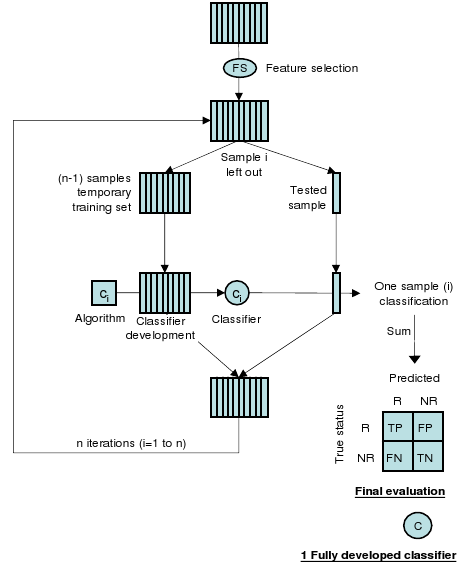
\includegraphics[%
    width=7.5cm,
    keepaspectratio]{dupuy3.png}
  \end{textblock*}
  \textblockcolour{white}
  \begin{textblock*}{43mm}(27mm,92mm)
    {\tiny(Dupuy and Simon, 2007, JNCI, 99)}
  \end{textblock*}

\note[item]{Ojo: tested NUNCA son vistos en training}
  
\end{frame}





\begin{frame}
\frametitle{CV and others}


\begin{itemize}
\item There are related techniques, such as bootstrap, etc.
\item To leave apart a single testing set is a bad idea.

\item Cross-validation: can have high variance.
\item Best approaches (?):
  \begin{itemize}
  \item A variant of CV (repeated splits, 50 times 10)
  \item Bootstrap (632+)
  \end{itemize}
% not clear.
% \begin{itemize}
% \item Molinaro, Simon, Pfeiffer. 2005. Bioinformatics, 21 (15): 3301-3307
% \item Braga-neto, Dougherty. 2004. Bioinformatics, 20 (3): 374-380.
\end{itemize}
\end{frame}



\begin{frame}
\frametitle{Classification, number of genes, etc}
And how do we choose the number of genes?

\vspace*{15pt}
Look, for example, at \Burl{http://tnasas.iib.uam.es}
\end{frame}




\begin{frame}
  \frametitle{We might not want to use many genes}
  \begin{itemize}
  \item Number of features (genes) vs.\ number of samples
  \item ``Metafeatures'' (metagenes):
    \begin{itemize}
    \item Biological relevance
    \item Statistical noise reduction (averages)
    \end{itemize}
  \item Adding not-very-relevant features generally decreases test set performance.
  \end{itemize}
\end{frame}


\begin{frame}
\frametitle{Validating what?}
\ldots what is it we are validating? how do we measure predictive ability?


\end{frame}


\subsection[Predictive ability]{Predictive ability}

% \begin{frame}
%  \tableofcontents[currentsection,subsectionstyle=show/show/hide]

% % \tableofcontents[currentsection]
%  \end{frame}


%\subsection{Sensitivity, specificity, etc}
\begin{frame}
\frametitle{Specificity and sensitivity}
\begin{center}

{\small
\begin{tabular}{l|cc}
 &\multicolumn{2}{c}{Predicted}\\
\hline
True & Diseased & Healthy\\
\hline
Diseased & True Positive (TP) & False Negative (FN)\\
Healthy & False Positive (FP) & True Negative (TN)\\
\hline
\end{tabular}
}
\end{center}


\begin{itemize}
\item Sensitivity $=\frac{TP}{TP + FN}$
\item Specificity $= \frac{TN}{TN + FP}$
\end{itemize}

\end{frame}


\begin{frame}
\frametitle{Error rates or predictive values?}
\begin{itemize}
\item (From van Belle, 2002, p. 96).
\item  Prevalence of colorrectal = 0.003
\item Hemoccult test: sensitivity: 50\%; specificity: 97\%.
\item I am positive!!!
\pause
\item The probability of having colorrectal cancer is only 5\%.
\item Eh?
\end{itemize}
\end{frame}

\begin{frame}
\frametitle{}
\begin{itemize}
\item I want to know: $P\left[Diseased|positive\right]$
\item Prevalence = $P(D)$
\item $P(D|p) = \frac{P(D \cap p)}{P(p)}$
\item $P(D \cap p) = P(p|D) P(D)$ (Bayes rule)
\item $P(p) = P(p|D) P(D) + P(p|D^c) P(D^c)$
\item $P(p|D) = TP/(TP + FN) = Sensitivity$
\item $P(p|D^c) = 1 - Specificity = FP/(FP + TN)$
\item $P\left[Diseased|positive\right] = $
$ = \frac{P(D) * Sensitivity }{P(D) * Sensitivity + P(D^c) (1 -
  Specificity)}$
\item $ P(D^c) = 1 - P(D) $
\end{itemize}
\end{frame}


\begin{frame}
\frametitle{}
\begin{itemize}
\item $\frac{\displaystyle 0.003 * 0.5}{\displaystyle 0.003 * 0.5 + 0.997 * 0.03} = 0.048$
\end{itemize}
\end{frame}

\begin{frame}
\frametitle{}
\begin{itemize}
\item $P\left[Diseased|positive\right] =$ Positive predictive value
\vspace*{15pt}
\item $P\left[Healthy|Negative\ test\right] =$ Negative predictive value $=$
$=\frac{(1 - P(D)) Specificity}{(1 - P(D)) Specificity + P(D) (1 - Sensitivity)}$
\vspace*{15pt}
\item Beware where prevalence estimate is coming
  from!!!!!
  % OJO de donde sale la estimación de la prevalencia!!!! (Comentario
  % al Suppl.\ 2 de Dupuy and Simon).
\end{itemize}
\end{frame}



\begin{frame}
\frametitle{ROC curves}
\begin{center}
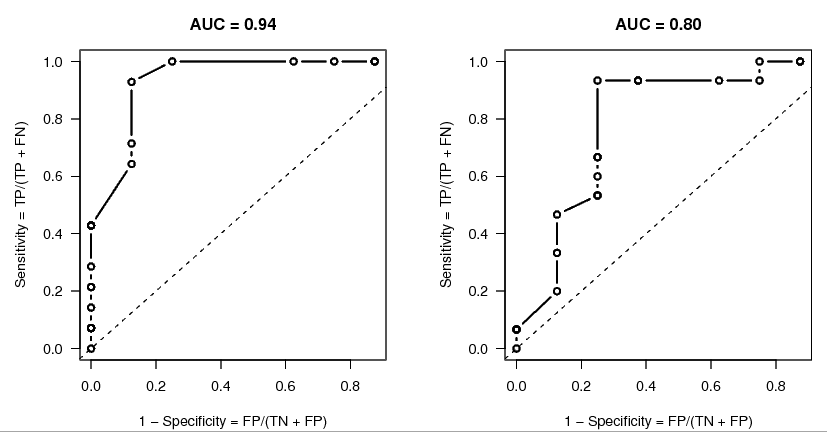
\includegraphics[%
    width=10.0cm,
    keepaspectratio]{ROC.png}
\end{center}
\end{frame}




%\subsection{Predictive ability}


% \begin{frame}[fragile=singleslide]
% \frametitle{Predictive ability?}
% {\small
% \begin{verbatim}
% Call:
% coxph(Surv(time, status) ~ clinical.score1 + 
%                            clinical.score2 + 
%                            our.risk.index)


%                         coef    z       p
% clinical.score1         3.74   2.55  0.011
% clinical.score2        -1.49  -3.17  0.001
% our.risk.index         -2.64  -2.51  0.012

% Likelihood ratio test= .... p=3.40e-07  n= 200
% \end{verbatim}
% }

% (Note: we have two different kinds of variables. We will return to that
% \hyperlink{covars}{\beamergotobutton{Clinical covariates}}
% \end{frame}


% % \begin{frame}
% % \frametitle{Capacidad predictiva?}
% % \begin{enumerate}
% % \item Identificamos 7 genes relevantes. 
% % \item Obtenemos índice de riesgo.
% % \item Ajustamos modelo de Cox con ese índice + el (los) mejor(es) indicador(es) clínico(s) convencional(es) X.
% % \item Si p-valor del índice es significativo: el nuevo índice es valioso
% % \end{enumerate}
% % \end{frame}




\begin{frame}
\frametitle{Predictive ability?}
\begin{itemize}
\item p-values, hazard-ratios, regression slopes, etc, are measures of
  association, not of predictive ability.
% \item Nuestra pregunta es: 
\vspace*{20pt}

\item Measuring predictive ability: how similar are predicted and observed?

\end{itemize}
\end{frame}



\begin{frame}
  \frametitle{Proportion correctly classified}
  \begin{itemize}
  \item Probably NOT what you want.
  \item Easily ``game-able''.(From posts by Frank Harell)
    \begin{itemize}
  \item You can manipulate the proportion classified correctly in a number
    of silly ways. The easiest way to see this is if the prevalence of Y=1
    is 0.98 you will be 0.98 accurate by ignoring all the data and
    predicting everyone to have Y=1.
  % \item Another way to saying all this is that by changing from an
  %   arbitrary cutoff of 0.5 to another arbitrary cutoff, different
  %   features will be selected. An improper scoring rule is optimized by a
  %   bogus model.
    \end{itemize}
  \item And we have not even considered asymmetric costs of mistakes.
  \end{itemize}
\end{frame}


\begin{frame}
\frametitle{Measuring predictive ability}

\begin{description}

\item[Brier score] related to $\Sigma_i (Y_i - q_i)^2$, where
$Y_i$ is the real status (e.g., class A vs. class B ---if A = 1, if
B = 0)  and $q_i$ is the predicted probability of being of class A.


\item[Concordance index (C-index)] Probability that, for all pairs of subjects
  where one is of one kind and the other of another kind, the patient with
  larger predicted probability of being of class A is really A. Related to
  ROC curves (later).

\item[Area under ROC curve] As it says: area under ROC curves 

\end{description}

Beware: Brier score, C-index, ROC: using ``out of bag'' predictions!!

\end{frame}



% \begin{frame}
% \frametitle{Measuring predictive ability}
% \begin{itemize}
 
% \item Area under ROC curve (in a moment)

% % \vspace*{20pt}
% % \item Survival data: active research areas
% % %% \item (More later \hyperlink{brierscore}{\beamergotobutton{Predicted and observed}}).
% \end{itemize}


% Beware: Brier score, C-index, ROC: using ``out of bag'' predictions!!



% \note[item]{Lo que he contad no es facil de implementar ni llevar a cabo}
% \note[item]{No creo que se peuda ni con Excel ni con SPSS.}
% \note[item]{No hay más remedio que poner un estadístico en nuestra vida. ¿Cuándo?}

% %% FIXME: explicar eso?

% \end{frame}


\section[Survival]{Survival analysis}

\begin{frame}
  \frametitle{Lots of data are survival data}
  \begin{itemize}
  \item Time until I have to change the light bulb of my living room.
  \item Time until death.
  \item Time until \ldots
  \item (no, not everything qualifies).
  \end{itemize}
\end{frame}



\begin{frame}
\frametitle{Introduction to survival models}
\begin{itemize}
\item Time until ``failure'' (death, relapse, change of state, etc)
\item Often censored:
  \begin{itemize}
  \item We observe $\min(T, c)$  where T is life duration, time to death, and
  c the ``censoring time''.
  \end{itemize}
\item Distributions such as exponential, weibull, etc
\item We should NOT discretize nor use linear regression. \textbf{Use
    methods that are appropriate for the type of response}
% \item More details under \hyperlink{Survival}{\beamergotobutton{Appendix:
%       Survival analysis with genomic data}}
\end{itemize}
\end{frame}



\begin{frame}
  \frametitle{Buzz words to remember}
  \begin{itemize}
  \item \textbf{Cox model}: like a linear model but we model hazard rates ($h(t)$,
    ``instantaneous rate of death at $t$ given that you are alive at $t$.'')
  \item \textbf{Parametric survival models}: model the distribution of
    time to death.
  \item \textbf{Log-rank test}: a way of comparing survival curves. \Burl{http://signs2.iib.uam.es/Examples/CommentedExample/results.html}
  \end{itemize}
\end{frame}




\begin{frame}
  \frametitle{Cross-validation, estimating predictive ability, etc}
  \begin{itemize}
  \item All we have seen before applies.
  \item Estimating predictive ability is more complicated.
  \item Different criteria and different weights at different times (early
    vs.\ late events, for example).
  \end{itemize}
\end{frame}


\begin{frame}
  \frametitle{Tools}
  \begin{itemize}
  \item Not many.
  \item Beware of possible issues in the evaluation of predictive performance.
  \item \Burl{http://signs2.iib.uam.es}
  \end{itemize}
\end{frame}

\section[Added value]{Does this add anything?}
% \subsection{Models to build}
% \begin{frame}
% \frametitle{Models to build}

% We will want to build the following:

% \begin{itemize}
% \item A model/algorithm/signature with the genomic data. There are many
%   options. 
%   \vspace*{20pt}

% \item A model just with clinical covariates (or maybe just follow the
%   recipe for a know method of building ``usual risk scores'').

% \vspace*{20pt}

% \item A model with the usual clinical indicators + genomic data. BEWARE:
%   no selection/penalization/regularization with the clinical indicators.

% \end{itemize}

% \end{frame}


% \subsection{And the additional covariates?}
\begin{frame}[label = covars]
\frametitle{Clinical covariates}
\begin{itemize}
\item We often have clinical covariates
\item How are we to include that info?
\item Frequently predictors based on other indices
\item Does gene expression improve prediction?
\item Key question: \mg{Does using gene expression add anything? Is it
    worth it?}
\item \textbf{Does the new method/algorithm, based on genomic data,
    improve our ability to predict a result, compared to what we could
    predict without those genomic data?}
\item Worth it \ldots for what? Clinical utility vs.\ basic knowledge.
%  (And issues of ``epistemic clarity'' and intellectual honesty).
\end{itemize}
\end{frame}


\begin{frame}
\frametitle{Why would predictions not improve with expression data?}
\begin{itemize}
\item Expression data can be just noise.
\item Expression data are redundant given the clinical covars. (which are
  often cheaper and faster to measure).
\item (BEWARE: no implication about causality. This is irrelevant in this
  predictive scenario.) 
\end{itemize}
\end{frame}


\begin{frame}
\frametitle{Reasons for caution}
\begin{itemize}
\item Truntzer et al. 2008.\textit{BMC Bioinformatics}, 9: 434. Survival
  data.
\item ``ability of the model to predict outcome with
  new datasets is overestimated'' with expression data. 
\item No optimism with clinical covars.
\item They are two very different kinds of variables.
\end{itemize}
\end{frame}


\begin{frame}
\frametitle{Simple solutions}
\begin{itemize}
\item \og{``Put everything in the same bag, and apply the usual methods''}
\item But ``Clinical covariates come first''
\item ``Same bag'' approach can affect negatively to clinical covars if
  they are correlated with gene expression.
\item Coefficients of clinical covars must be estimated without
  penalization. And a need if we want to compare with models that only
  have clinical covars
  (see Binder and Schumacher).
\item ``Litmus test'': if genes do not provide anything, final model
  should be as good as if it only had clinical covars (Boulesteix et
  al., 2008).
\end{itemize}
\end{frame}


\begin{frame}
\frametitle{Simple solutions (II)}
\begin{itemize}
\item \og{If there are discrete groups (sex, tumor marker) do separate analysis}
\item But we often have small sample sizes.
\item Does not answer the original question directly: do gene expression
  data improve anything?
\end{itemize}
\end{frame}

\begin{frame}
\frametitle{Simple solutions (III)}
\begin{itemize}
\item \og{Two classifiers: only with clinical covs.\ and only with gene
    expression data.}
\item We can compare models (though not obvious: they are not nested).
\item Does not answer the basic question.
\end{itemize}
\end{frame}


% \begin{frame}
% \frametitle{Simple solutions (IV)}
% \begin{itemize}
% \item \og{Use residuals}
% \item Adjust using clinical covs, as dictated by best practices.
% \item Take residuals
% \item See what gene expression provides.
% \item Buuuuut \ldots in many cases residuals are not obvious with some
%   type of data.
% \item Not obvious we are answering the original question.
%   % \item (La idea de ``residuo'' es implícita en muchos ajustes iterativos,
% %   ej., boosting, pero residuo está cuidadosamente elegido en el contexto
% %   del model fitting algorithm).
% \end{itemize}
% \end{frame}



% \begin{frame}
% \frametitle{Not so simple solutions}
% \begin{itemize}
% \item Boulesteix et al. 2008. \textit{Bioinformatics},
%   24:1698--1706. Classification (but they say  ``Our method is
%   easily generalizable'').
% \begin{itemize}
% \item PLS for gene expression: $\rightarrow T_L$.
%   % (using usando ``pre-validation'' ---como CV prediction) para gene
%   % expression: $\rightarrow T_L$
% \item Random forest with $T_L$ + clinical covs
% \end{itemize}
% \end{itemize}
% \end{frame}



\begin{frame}
\frametitle{Not so simple solutions}
\begin{itemize}
\item Do not penalize or remove clinical covariates.
\item Adjust for those.
\item Then add ``omics'' data.
\item Assess if omics data adds something to previous model with only
  clinical covariates.
\end{itemize}

% {\scriptize
% \begin{itemize}
% \item Binder and Schumacher. 2008. \textit{BMC Bioinformatics}, 9:
%   14. Survival data.
%   \begin{itemize}
%   \item Boosting of Cox model
%   \item Clinical covs not penalized
%     \item See also B. Johnson, 2009. \textit{Biostatistics}: accel.\
%       failure time model. Clinical covars enter non-linearly. Genetic
%       features enter linearly after adjusting for clinical covars.
%   \end{itemize}

% \item Boulesteix and Hothorn, 2010. \textit{BMC
%     Bioinformatics}. GLM for clinical covariates; then boosting for gene
%   expression data. Assess added value by permutation tests.
% \end{itemize}
% }
\end{frame}



\begin{frame}
\frametitle{Conclusions (?)}
\begin{itemize}
\item Many reasonable methods with similar solutions. Includes methods
  that are rather straightforward (DLDA, KNN).
% \item Por qué la penalización no se ha hecho aun más popular? (Lasso,
%   L2Boosting, elastic net, etc)
\item Instability and multiplicity of solutions: are they a problem?
\item Which is the best number of genes is difficult to tell.
\item Why are we doing this? Biological interpretation/understanding or
  for diagnostic test development?
\end{itemize}
\end{frame}


%% FIXME
%% mention this in class
%% why you do not need many features

%%\section[Classif.summary]{Classification/prediction: summary}

\section[Clustering]{Are there groups? Clustering}

 % \begin{frame}
 % \tableofcontents[currentsection,subsectionstyle=show/show/hide]
 % \end{frame}



%\subsection{Are there groups?}

\begin{frame}
\frametitle{Are there groups?}
\begin{itemize}
\item Can we find groups of genes that behave in a similar way, but
  different from other genes?
\item Likewise for subjects?
\end{itemize}

``Class discovery'', clustering.


\end{frame}


\begin{frame}
\frametitle{Only makes sense if $\ldots$}
\mg{we do not know, before hand, that there are different groups of genes/subjects}.

\end{frame}


%\subsection{Two pieces}


\begin{frame}
\frametitle{Two needed pieces}

What does it mean to ``behave similarly'' and measuring similarity.
\vspace*{20pt}

Describing how we will group based on those similarities.

\end{frame}



%\subsection{Similarity}

\begin{frame}
\frametitle{First piece: similiarity (or ``dis-similarity'')}
\begin{itemize}
\item Distances (e.g., Euclidean distance).
\item Correlations.
\end{itemize}
\end{frame}


\begin{frame}
  \textblockcolour{}
\begin{textblock*}{105mm}(20mm,11mm)
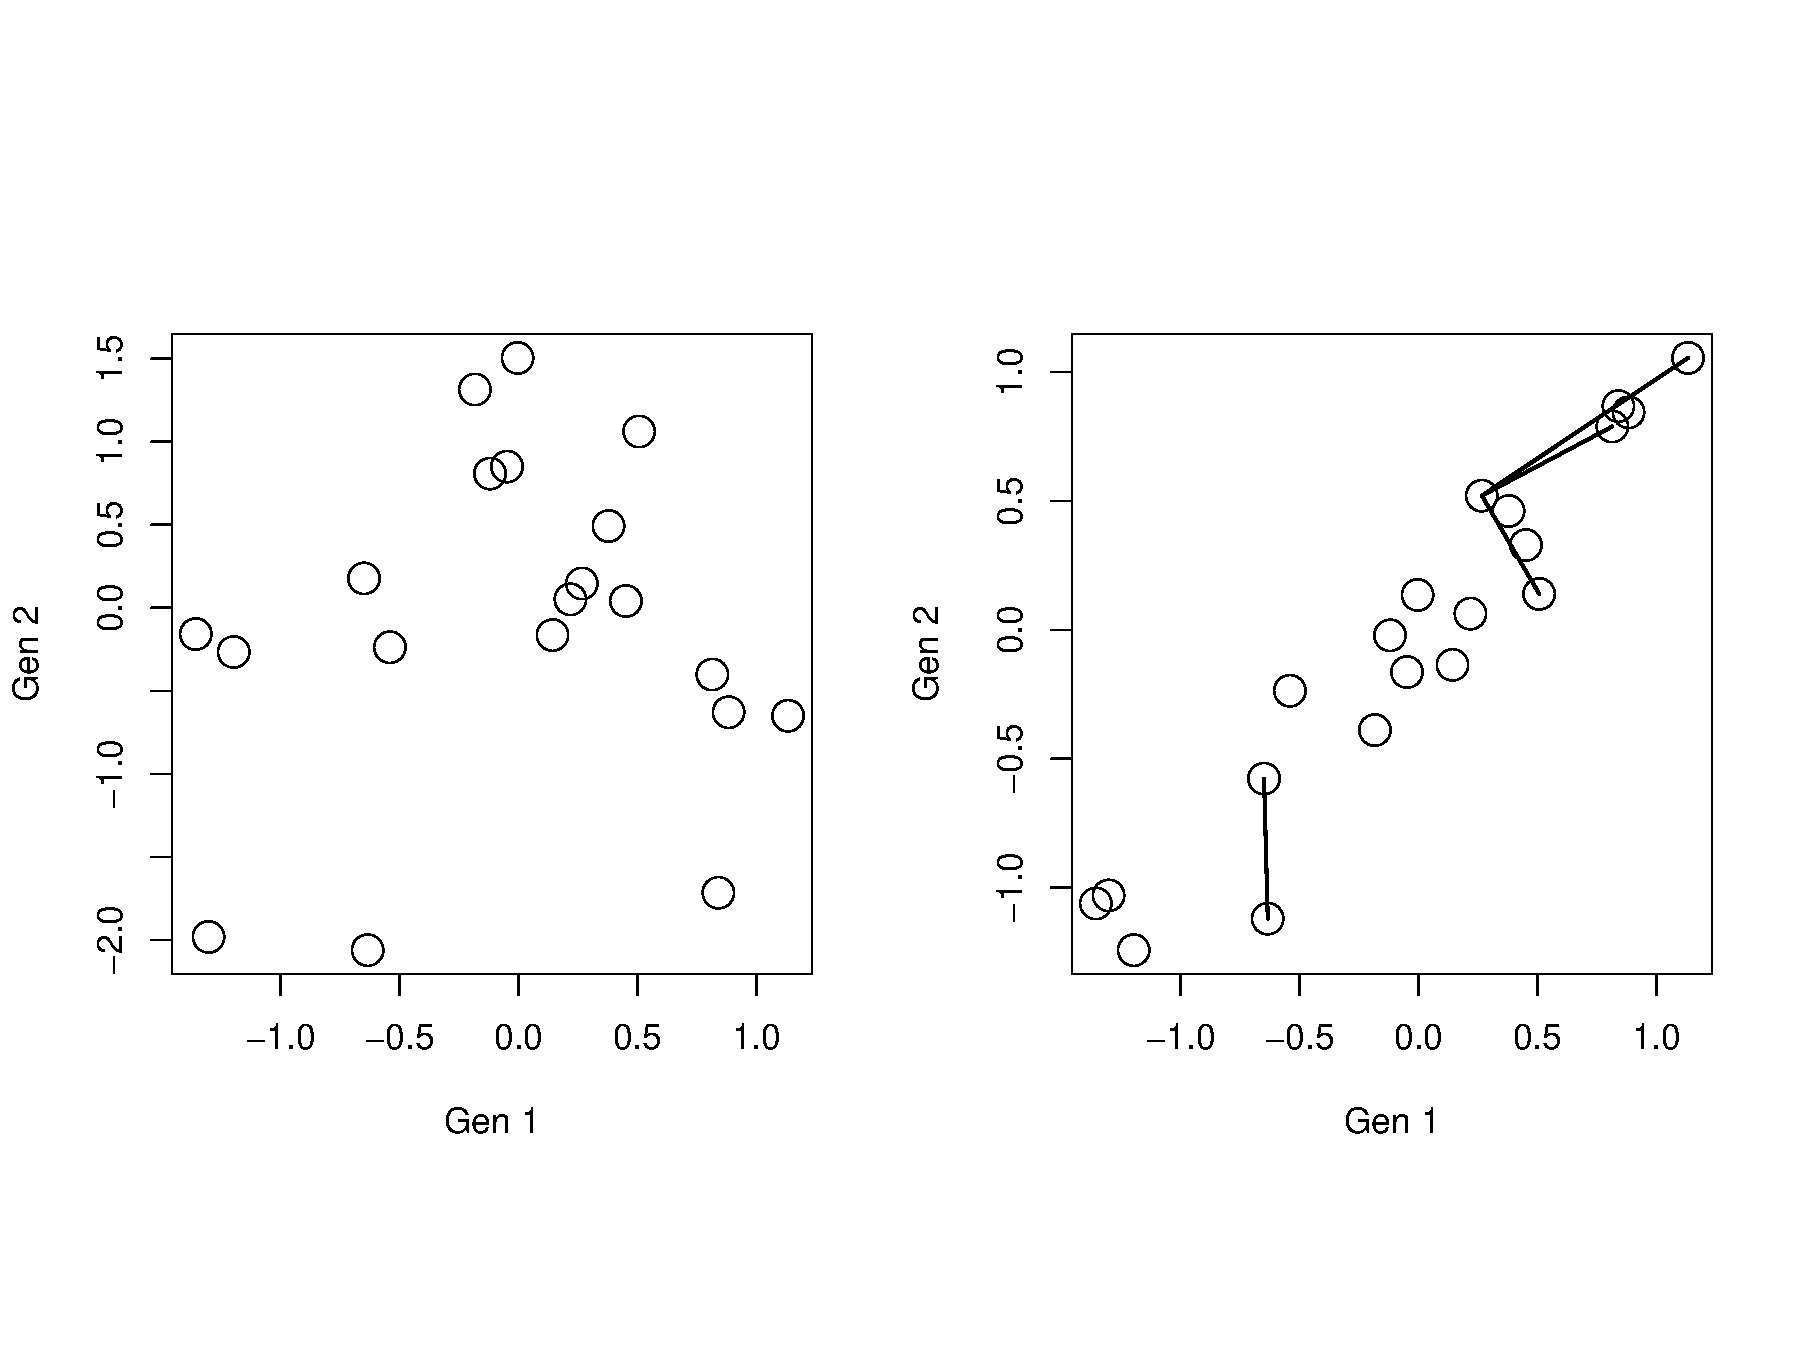
\includegraphics[%
    width=10.5cm,
    keepaspectratio]{cluster.pdf}
\end{textblock*}
\end{frame}



\begin{frame}
\frametitle{}

We end with a matrix of similarities between all pairs of subjects or genes.

\vspace*{14pt}
Now what?



\end{frame}



\begin{frame}
\frametitle{}

\begin{center}
\begin{tabular}{c||c|c|c|c|}
   &   s1   &   s2   &    s3   &   s4 \\
\hline
\hline
s1 &   -    &   2    &     7   &    3 \\
\hline
s2 &   -    &   -    &     8   &    4 \\
\hline
s3 &   -    &   -    &     -   &    9 \\
\hline
s4 &   -    &   -    &     -   &    - \\
\hline
\end{tabular} 

\end{center}
\vspace*{12pt}

\centerline{???}


\end{frame}






%\subsection{Clustering algorithms}

\begin{frame}
\frametitle{Second piece: clustering algorithms}
\begin{itemize}
\item Hierarchical:
\begin{itemize}
\item Divisive
\item Agglomerative (UPGMA again!!!)
\end{itemize}
\item No hierarchical (need to specify number of clusters).
\end{itemize}
\end{frame}






% \begin{frame}
% \frametitle{Jeraquicos (e.g., aglomerativos)}
% \begin{itemize}
% \item Juntar los dos que tengan menor dis-similaridad (i.e., estatura mas
%   parecida).
% \item Continuar juntando, hasta que todas las muestras (todos los sujetos) en algún grupo.
% \pause
% \item ¿Cómo continuar juntando? La nueva muestra, ¿a quien se tiene que
%   parecer? 
% \end{itemize}

% \end{frame}

% \begin{frame}
% \frametitle{No jerárquicos}
% \begin{itemize}
% \item Sospechamos que existen dos grupos.
% \item Encontrar la asignación de todos los elementos a dos grupos de
%   forma que ``sea la mejor solución''. Por ejemplo: la suma de distancias
%   de cada observación a su ``centro del cluster'' sea mínima..

% \vspace*{12pt}
% \item (La matriz de distancias entre puntos no nos hace falta; sí, en este
%   caso, de los puntos al centro del cluster).
% \end{itemize}
% \end{frame}


% \begin{frame}
% \frametitle{Ejemplo}
% Ver si existen grupos en esta clase en función de la estatura.
% \end{frame}


% \begin{frame}
% Estatura: ya tenemos algo definido, que es la estatura.

% Podemos definir distancia entre sujetos como la diferencia en estatura.
% \end{frame}



%\subsection{Problems}

\begin{frame}
\frametitle{Problems ...}
\begin{itemize}
\item What measure of similarity should we use?
\item What is the appropriate clustering algorithm?
\item Should we use all genes when we cluster subjects?
\end{itemize}
\end{frame}



\begin{frame}
\frametitle{Precautions}
\begin{itemize}
\item Clustering is class discovery: it is an exploratory tool, not a
  confirmatory one.
  
\item Clustering ALWAYS returns clusters, whether or not there is any real
  structure. 
\item If a cluster is ``relevant'' and ``stable'' is a different question.
\item Clustering is not the right tool if we know about groups before hand.
\end{itemize}
\end{frame}


\begin{frame}
\frametitle{t-test and cluster}
What do you think about the idea of doing clustering and then a t-test?
\end{frame}


\begin{frame}
\frametitle{An interesting idea: searching for transcription factors}
\begin{itemize}
\item Cluster genes
\item Search in up-stream regions for the most frequent l-mers

\item (Details and references in Cristianini and Hahn 2006 and Harmer et
  al. 2000.)
\end{itemize}
\end{frame}


\begin{frame}
  \frametitle{And there is biclustering}
  \begin{itemize}
  \item Cluster according to both dimensions, at the same time.
  \end{itemize}
\end{frame}




\section{Appendix: survival analysis}
\begin{frame}[label=Survival]
\frametitle{Appendix: Survival analysis with genomic data}
\begin{itemize}
\item Many methods suggested
\item Few comparisons that settle the issue
\item How do we compare performance? How do we assess model quality?
\end{itemize}
\end{frame}



\begin{frame}
\frametitle{}
\begin{itemize}
\item We observe $\min (T, c)$ where T is life duration, time to death, and
  c the ``censoring time''. $F(t)$: cumulative distr.\
  function of X.
\item $F(t) = P(T \le t) = \int_0^t f(x) dx$
\item Survival function, $S(t)$:
  probability of being alive at time $t$. 
\item $S(t) = 1 - F(t) = \int_t^{\infty} f(x) dx$.
\end{itemize}
\end{frame}

\begin{frame}
\frametitle{}
\begin{itemize}
\item ``hazard function'', $h(t)$: instantaneous rate of death
\item $h(t) = \lim_{\Delta t \rightarrow 0^+} \frac{P(t \le T < t +
      \Delta t | T \ge t)}{\Delta t} $
%%$ = \frac{S(t) - S(t + \Delta t)}{S(t) \Delta t}$
\item $h(t) \Delta t$ = probability of dying in the interval
   $\left[t, t + \Delta t \right]$, given that the subject is alive at
   time  $t$
\item $f(t) = \lim_{\Delta t \rightarrow 0^+} 
\frac{P(t \le T < t + \Delta t)}{\Delta t} = 
\frac{dF(t)}{dt} = - \frac{dS(t)}{dt} $
\item $h(t) = \frac{f(t)}{S(t)}$
\end{itemize}
\end{frame}


\begin{frame}
\frametitle{}
\begin{itemize}
\item Cumulative hazard: $H(t) = \int_0^t h(u)du = -\log(S(t))$
\item $S(t) = 1 -F(t) = P(T \ge t) = \exp(-H(t)) = exp(-\int_0^t h(u)du)$
% \item $\hat{S(t)} = \frac{\mathrm{number of subjects alive at }
%     t}{\mathrm{número total de sujetos}}$
\item Median survival time: 
\begin{itemize}
\item time beyond which 50\% of the subjects of the cohort are expected to
  be alive.
\item The first $t$ where $\hat{S}(t) \le 0.5$
\end{itemize}
\item Mean survival time:  $\int_0^{\infty} t f(t) dt$. But censored data
  create problems. Several approaches, e.g.,
  ``Efron's tail correction''. 
\end{itemize}

\end{frame}



\begin{frame}
\frametitle{Kaplan-Meier estimator}
\begin{itemize}
\item $n_i$: number of cases at risk just before time $t_i$ (i.e.,
  those that are part of the study and are still alive and not censored at
    $t_i$).
\item $d_i$: the ones who die in the interval $i$.
\item Kaplan-Meier estimator: $\hat{S}(t) = \Pi \frac{n_i - d_i}{n_i}$
\end{itemize}
\end{frame}



\begin{frame}[fragile]
\frametitle{}

{\small \verb-T = 9, 13, 13+, 18, 23, 28+, 31, 34, 45+ -

\begin{verbatim}
 time n.risk n.event survival
    9      9       1    0.889
   13      8       1    0.778
   18      6       1    0.648
   23      5       1    0.519
   31      3       1    0.346
   34      2       1    0.173
\end{verbatim}
}


\begin{itemize}

\item $S(0) = 1$
\item $S(9) = \hat{S}(0) * (9 - 1)/9 = 0.889$
\item $S(13) = \hat{S}(9) * (8 - 1)/8 = 0.778$ (Note that there are 8 at
  risk and the one that dies has survival 13).
\item $S(13+) = \hat{S}(13+) * (7 - 0)/7 = 0.778$ (Note that there is no
  death event here).
\end{itemize}
\end{frame}


\begin{frame}
\frametitle{Log-rank test}
\begin{itemize}
\item One of the several ways to compare two or more survival curves.
\item Related to categorical data analysis by strata: like a
  Mantel-Haenszel test where each stratum is each period.
\item $H_0$: survivals are equal.
\item Compute a ``pooled sample estimator'' of number of events and number
  at risk  ($d_i$ y $n_i$ from before).
\item Compute differences between observed and predicted (ej.,
  $(d_{i1}/n_{i1}) - (d_{i}/n_{i})$.
\item Compute variance of those expected values.
\item Sum over all periods, weighted by $i$ (log-rank: weight
  = 1).
\item Compare with appropriate distribution (Z, Chi if $MH^2$).
\end{itemize}
\end{frame}


\begin{frame}
\frametitle{Cox Model}
\begin{itemize}
\item $h(t) = h_0(t) \exp(\beta_1 x_1 + \beta_2 x_2 + \ldots + \beta_q x_q)$
\item $h_0(t)$ : baseline hazard function. Common, independent of 
  $x$.
\item $\beta_i$: the effect of the given covariate (e.g.., gene $x_i$) on 
  $h(t)$.
\item Hazard ratio is constant:
  $\frac{h(t|\mathbf{x}_1)}{h(t|\mathbf{x}_2)} =
  \frac{exp(\beta^T\mathbf{x}_1)}{exp(\beta^T\mathbf{x}_2)} = $
$ \frac{exp(\Sigma \beta_i x_{1i})}{exp(\Sigma \beta_i x_{2i})} = 
  exp(\Sigma \beta_i (x_{1i} - x_{2i}))$
\end{itemize}
\end{frame}


\begin{frame}
\frametitle{}
\begin{itemize}
\item Estimating $\beta$ is what matters. The $h_0$ is ignored (``Partial likelihood'').
\item Likelihood depends only on the ranking of the times to death (``non-parametric'').
\item To obtain predictions of time to death the  $h_0$ is estimated with
  another procedure.
\item ``Linear scores'' (``prognostic index''): $\hat{\beta^T}\mathbf{X}$
\item $\log(h(t)) = log(h_0(t)) + \beta_1 x_1 + \beta_2 x_2 + \ldots + \beta_q x_q$

\end{itemize}
\end{frame}




\begin{frame}
\frametitle{Other models}
\begin{itemize}
\item General: model time to death (or a transformation of time to death, such
  as $\log(time)$) as a function of covariates (and that function could
  be, e.g., and exponential).
\item Regression models using Weibull, exponential, etc.
\item Less used than Cox (need to chose scale parameters).
\item No proportional hazards assumption, and some times more flexible.
\item Not very much used with gene expression data. (But see Schmid y
  Hothorn, 2008, \textit{BMC Bioinformatics}, 9: 269).
\end{itemize}
\end{frame}



\begin{frame}
\frametitle{How to assess predictive abilities?}
\begin{itemize}
\item Censored: simple correlation observed-predicted will not work.
\item Continuous data: we cannot discretize.
\end{itemize}
\end{frame}


\begin{frame}
\frametitle{Not great ideas}

\begin{itemize}
\item Log-rank test between groups formed from predictions? Why is it a
  bad idea?
\pause
\item Mentioned in Dupuy and Simon: categorization, chi-square not valid.
\vspace*{10pt}
\pause
\item Survival model on the linear score, and assess slope (and its
  p-value). Why bad idea?
\vspace*{10pt}
\pause
\item Bovelstad et al., van Wieringen et al., Haibe-Kains et al., use
  questionable approaches.

\item (Yes, SignS implements a few bad ideas  $\ldots$).
\end{itemize}
\end{frame}



\begin{frame}[label=brierscore]
\frametitle{Predicted and observed: better ideas}
(Suggestion: read quickly)

\begin{description}
\item[$R^2$ extended to survival data]: $R^2 = 1 -
  exp(-\frac{2}{n}(l(\hat{\beta}) - l(0)))$ (similar to deviance)

\item[Brier score] related to $\Sigma_i (Y_i(t) - q_i(t))^2$, where 
$Y_i(t) = 1$ if subject $i$ is alive at $t$, $Y_i(t) = 0$ o.w., and 
$q_i(t)$ is the probability of surviving until  $t$ of subject $i$ (and
this we obtain from Cox model).

Brier score integrates over all  $t$.
\end{description}
\end{frame}


\begin{frame}
\frametitle{}
\begin{description}
\item[Concordance index (C-index)] Probability that, for a pair of
  patients chosen at random, the one with higher risk really dies
  earlier. Related to ROC curves.
  
\item[ROC curves] The cutoff is the risk score (or the linear
  predictor). The event is ``dead''. For each time $t$ we can compute the
  sensitivity and specificity as we move the cutoff. Then, compute area
  under the curve. Finally, integrate that AUC for all $t$.
\end{description}

Again: Brier score, C-index, ROC: using ``out of bag'' predictions!!

\end{frame}


\begin{frame}
\frametitle{}
\begin{itemize}
\item There are yet other measures. Those are the most widely used.
\item Which is best? What if method A is best with C-index and method B
  with Brier?
\item A recurrent theme: \textbf{survival analysis is complicated}. Thus,
  \textbf{shortcuts are unlikely to work} (only with good weather and if
  you know the area).
\end{itemize}
\end{frame}




% \begin{frame}
% \frametitle{Reviews}
% \begin{itemize}
% \item vanWieringen et al. 2008. \textit{Computational
%     Statistics and Data Analysis}, in press.
% \item Bøvelstad et al. 2007. \textit{Bioinformatics}, 23(16):2080-2087
% \item Schumacher et al. 2007. \textit{Bioinformatics}, 23(14):1768-1774
% \end{itemize}
% \end{frame}


% \begin{frame}
% \frametitle{Some other reviews and papers}
% \begin{itemize}
% \item Haibe-Kains, 2008. \textit{Bioinformatics}, 24(19): 2200-2208
%   (univariate or simple models are best)
% \item Gui and Li. 2005. \textit{Bioinformatics}, 21 (13): 3001--3008
% \item Segal. 2006. \textit{Biostatistics}, 7(2): 268-285.
% \item Ma and Huang. 2007. \textit{Bioinformatics}, 23(4):466-472
% \item Other comments in Diaz-Uriarte, 2008, \textit{BMC
%     Bioinformatics}, 2008, 9:30.
% \end{itemize}
% \end{frame}

% \begin{frame}
% \frametitle{Conclusions}

% \begin{itemize}
% \item Penalization (L1, L2, Lasso, $L_2$boosting --Hothorn, Bühlman)
%   works well. Many methods and subfamilies.
% \item Random forest-based also good.
% \item SuperPC (Tibshirani and Bair) not as good.
% \item Cox based on forward, backward, etc: much worse.
% \item Little work on non-proportional hazards models.
% \end{itemize}
% \end{frame}




%%% Local Variables: 
%%% mode: latex
%%% TeX-master: t
%%% End: 
